 \paragraph{} Les test ont été effectués sur des matrices 7x7 dus aux limitations de contraintes dans la version étudiant de AMPL avec le solveur knitro (300 contraintes maximum).  De ce fait, nous nous sommes limités également au premier modèlé décrit dans l'article pour AMPL.

\paragraph{} Les résultats de la version mathématiques sont plus précis, mais plus lent (car la limite de contrainte nous empêche de l'optimiser). 


\begin{figure}
        \begin{minipage}{.5\textwidth}
        \subfloat[AMPL]{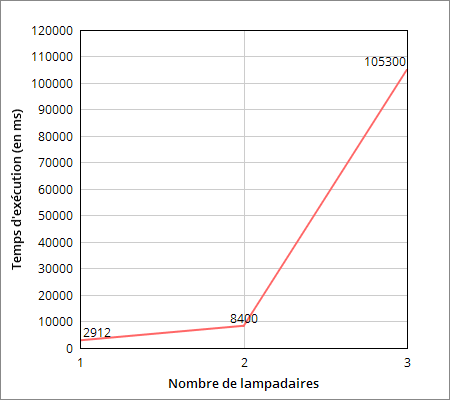
\includegraphics[scale=0.25]{./image/graphiqueAMPL.png}}
        \end{minipage}
        \begin{minipage}{.5\textwidth}
        \subfloat[Backtracking]{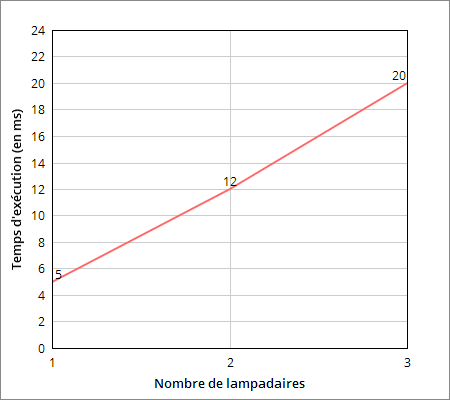
\includegraphics[scale=0.25]{./image/graphiqueBacktrack.png}}
        \end{minipage}
\end{figure}


\begin{figure}
        \begin{minipage}{.5\textwidth}
        \subfloat[Exemple de coloriage]{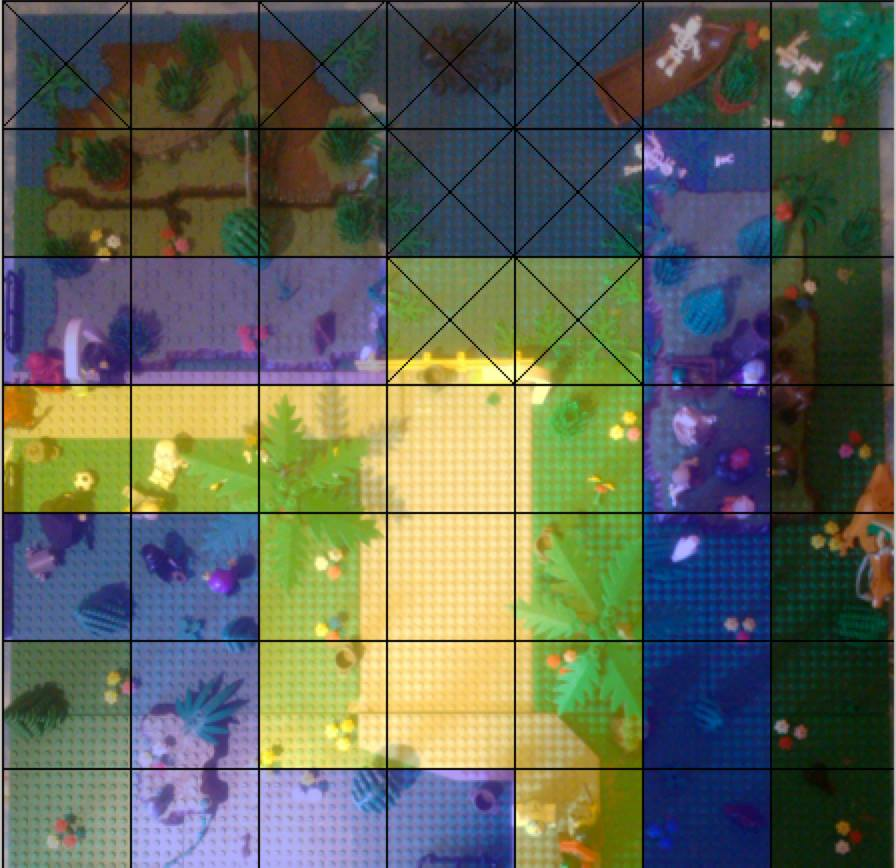
\includegraphics[scale=0.25]{./image/plateauColoriage1.jpg}}\par
         \subfloat[Résultat AMPL]{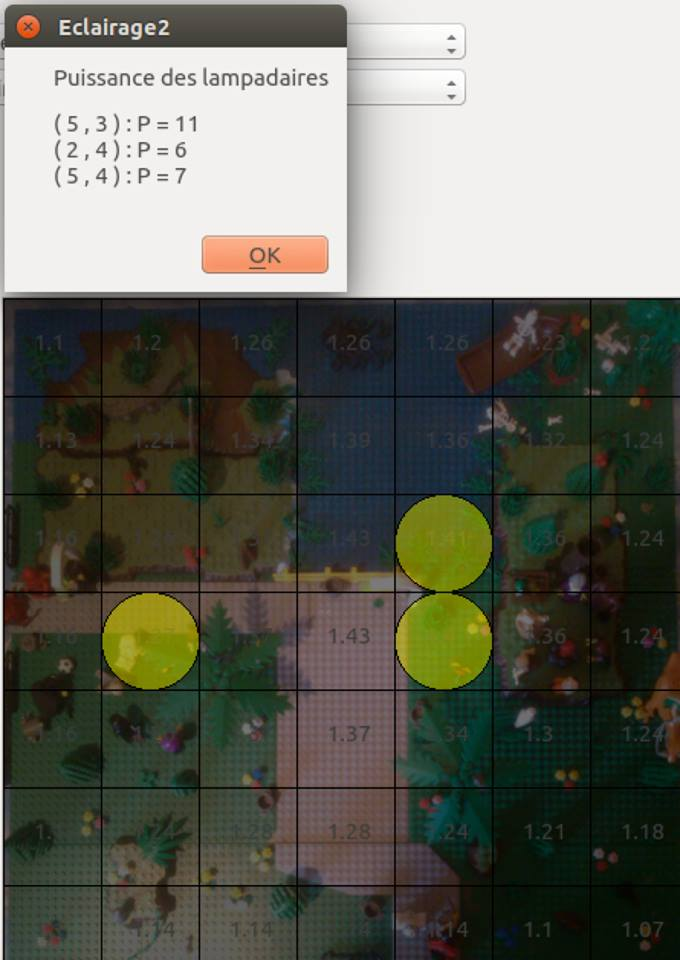
\includegraphics[scale=0.25]{./image/ampl1.jpg}}
        \end{minipage}
        \begin{minipage}{.5\textwidth}
        \subfloat[Résultat Backtracking]{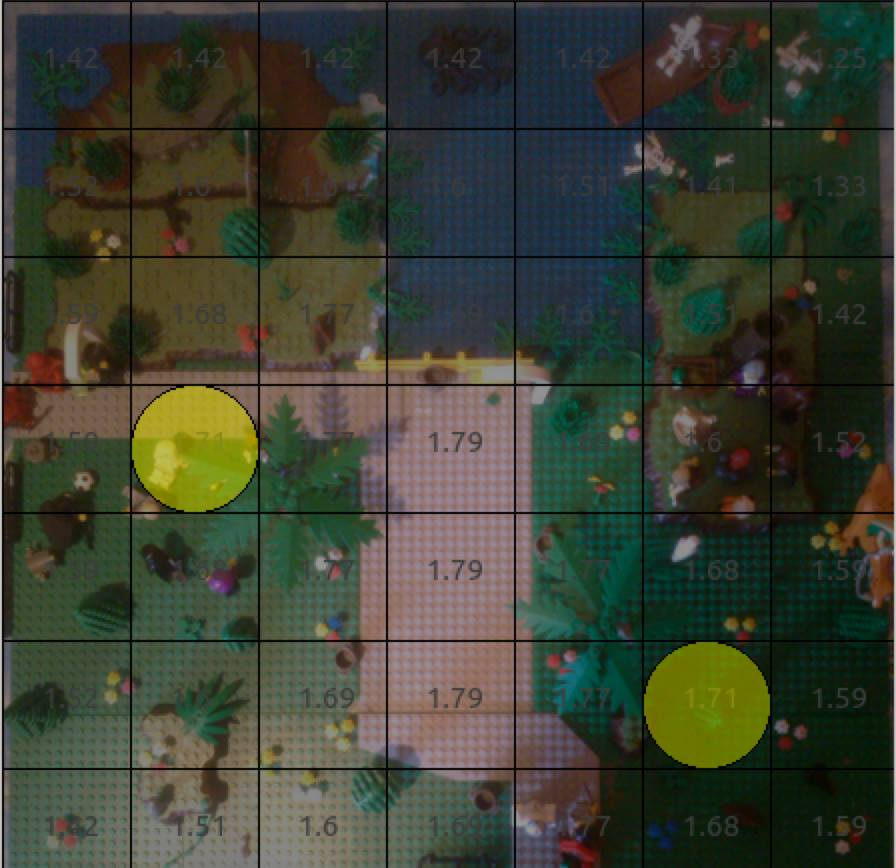
\includegraphics[scale=0.25]{./image/backtrack1.jpg}}\par
        \subfloat[Résultat Backtracking rapide]{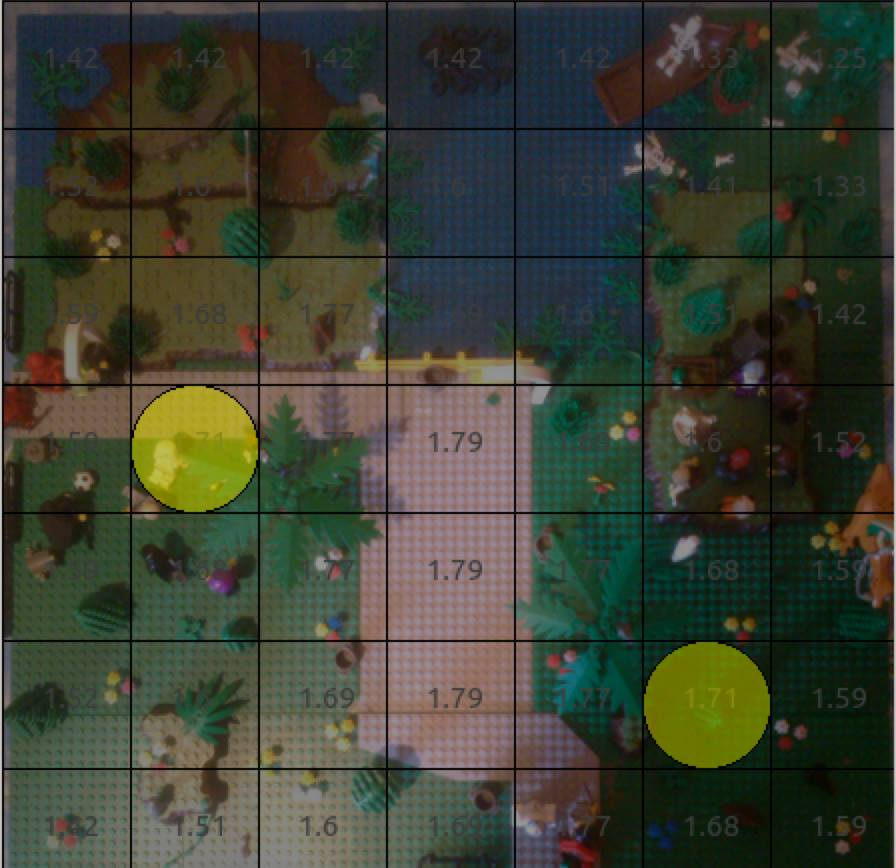
\includegraphics[scale=0.25]{./image/backtrackFast1.jpg}}
        \end{minipage}
\end{figure}

